%%%% --- CA --- %%%%
\section{Cellular Automata}
\label{methods:CA}
Cellular Automata (CA) consist of a discrete set of state machines called "cells," a set of possible states where these cells can be located, a fixed neighborhood of these cells to each other, and an update rule. 

For the update rule of a CA, in particular, \begin{enumerate}
    \item that it is executed in discrete time steps,
    \item that the state of a cell $x_{n,m}$ in the next time step $t+1$ is only determined by the states of the cell itself and its direct neighbors in this time step $t$ and
    \item that all cells execute the same update rule.
\end{enumerate}

The founder of CAs is \autocite{vonNeumann:1951}, who used it to try to model self-replicating artificial systems \autocite{Kari:2005:CA_survey}. CAs are used in many scientific disciplines to model non-linear systems \autocite{Pade:2023:HirarchicalNCA}. CAs themselves form a Turing-completed system, but in contrast to Turing machines, all cells calculate in parallel \autocite{Berto:StanfordSurvey_CA:2022}. For example, a more comprehensive survey on CAs can be found at \autocite{Berto:StanfordSurvey_CA:2022}.

As a simple example for visual data, one can imagine the pixels in an image. Then, for example, each pixel can be defined as a cell, the color or gray values of the pixels as the states, and, using the position of the pixels in the image as the neighborhood, e.g., each 3x3 field forms the neighbors of the middle pixel of this field.

The update rule can then be formulated as a 3x3 kernel. Two such examples are given in \ref{fig:ca_exp}. For (1) and (2), the following simple kernels and zero-padding were used: the initial state is on the far left, and the time steps to the right increase by 1:
\begin{align*}
    (1)\    \begin{bmatrix}
                1 & 0 & 0\\
                0 & 0 & 0\\
                0 & 0 & 0
            \end{bmatrix}
            \ , \qquad
    (2)\    \begin{bmatrix}
                0   & 0.5 & 0\\
                0.5 & 0   & 0\\
                0   & 0   & 0
            \end{bmatrix}\\
\end{align*}


\begin{figure}[h!]
    \centering
    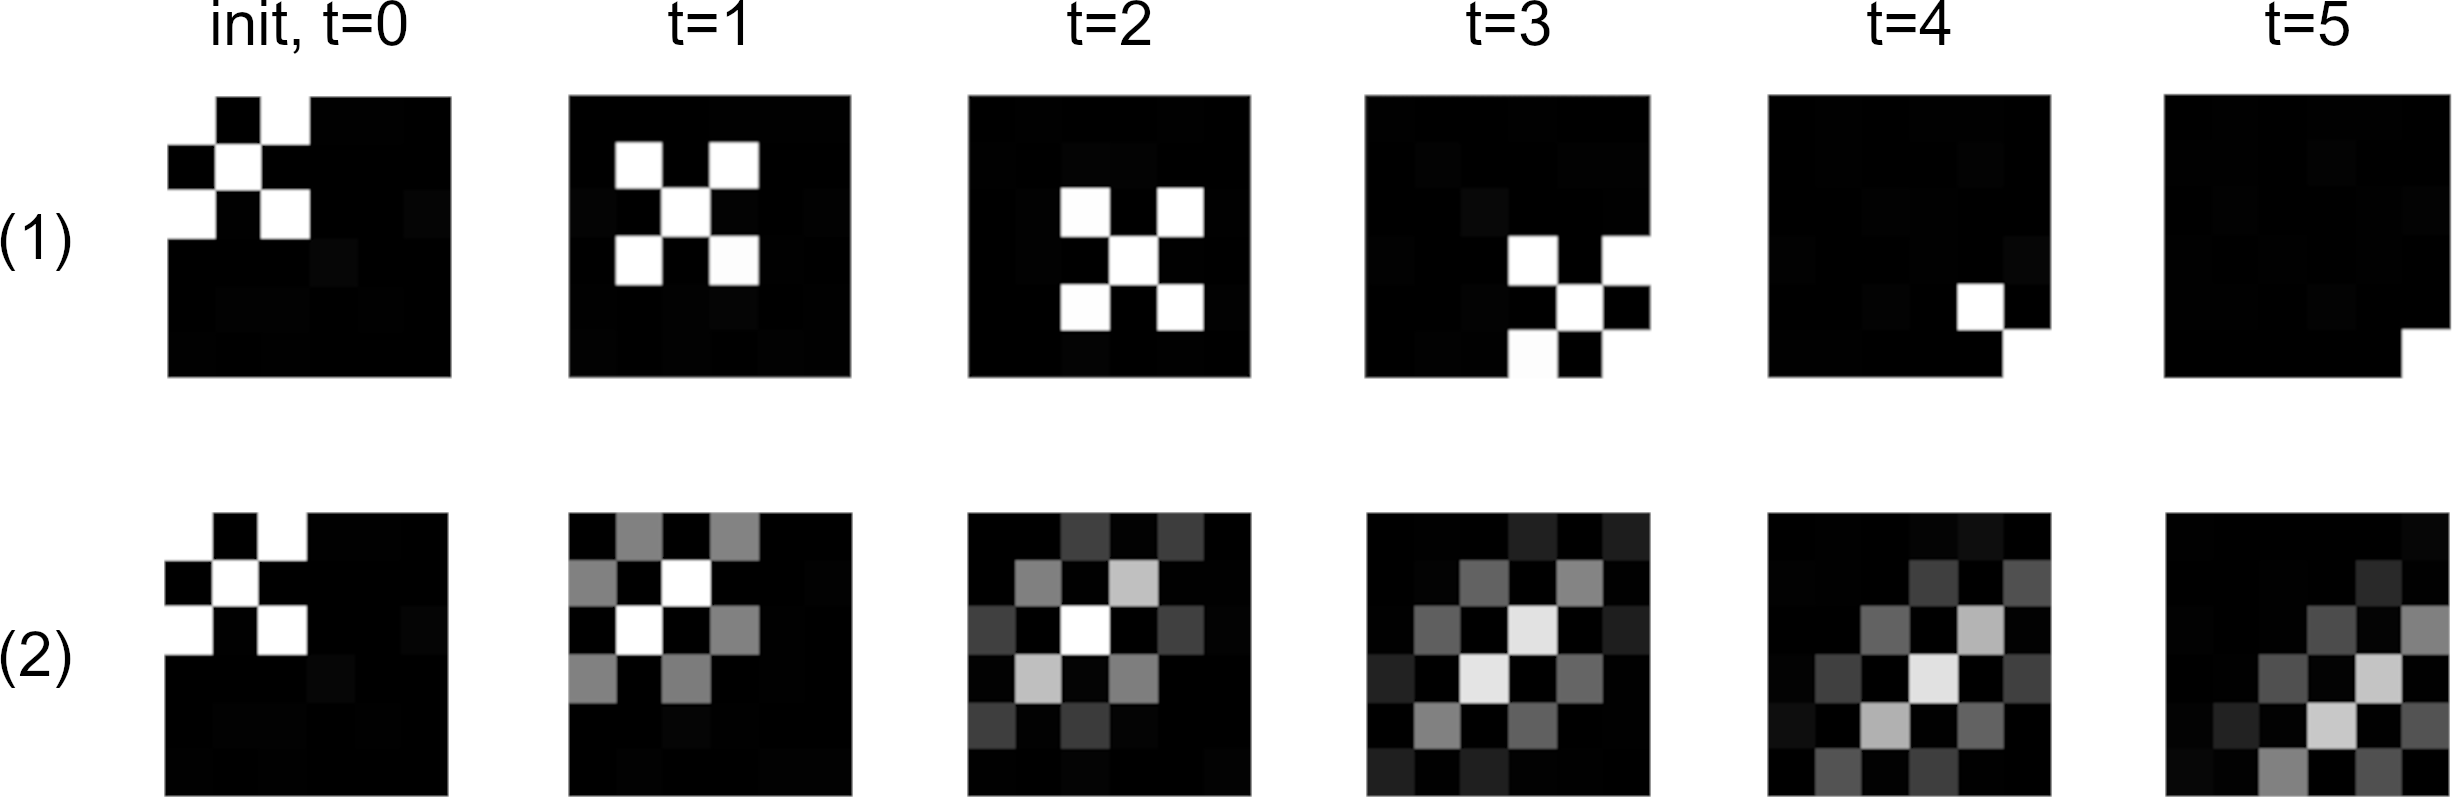
\includegraphics[width=0.9\linewidth]{Graphics/CA_examples.png}
    \caption{Examples of two elementary Cellular Automata on visual data. In a cellular automaton, the state of each cell (e.g., a pixel here) at time step $t+1$ is determined only by the states of the cell itself and its immediate neighbors at time step $t$. In this case, the 3x3 surrounding pixels. The update rules can be described as simple 3x3 kernels. Where time runs from left to right, and the filter is applied to each pixel in each time step. In example (1), there is only a simple shift, and in example (2), the original shape diverges and moves.}
    \label{fig:ca_exp}
\end{figure}

CAs are generally more complex than these simple examples and are not limited to visual data. Instead, among many other things, CAs can be used to simulate and model, e.g., urban evolution, turbulence phenomena, and other fundamental physics, and in general, many discrete dynamical systems, see, e.g., \autocite{Berto:StanfordSurvey_CA:2022}.

Thus, CAs exist for a long time and have a vast application potential. However, the main challenge in directly modeling CAs is often finding a suitable update rule \cite{Gilpin:2019:IntroduceNCA}. In Neural Cellular Automata, these update rules are modeled or trained with a neural network, which is discussed in more detail in the following section.